\documentclass[crop,border=0pt]{standalone}

\usepackage{mathtools}
\usepackage{tikz}
\usetikzlibrary{positioning,scopes,arrows}

\begin{document}
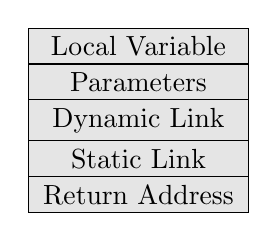
\begin{tikzpicture}[
  mybox/.style={
    fill=gray!20,
    minimum width=2.8cm,
    minimum height=1em,
    inner sep=3pt,
    draw},
  node distance=-\pgflinewidth]
  \node [mybox] (b0) {Local Variable};
  \node [mybox, below=of b0] (b1) {Parameters};
  \node [mybox, below=of b1] (b2) {Dynamic Link};
  \node [mybox, below=of b2] (b3) {Static Link};
  \node [mybox, below=of b3] (b4) {Return Address};
\end{tikzpicture}
\end{document}
